\title{Synthesizing Static Analyses from Examples}
\author{
        Martin Kellogg \\
        University of Washington
            \and
        Everett Maus\\
        Microsoft Corporation
}


\documentclass[10pt,conference]{IEEEtran}

\usepackage{graphicx}
\usepackage{myref}
\usepackage{booktabs}
\usepackage{url}

\begin{document}

\maketitle

\begin{abstract}

Constructing static analyses requires a great deal of
manual, expert programmer effort. Because of the large amount of
effort required to build a precise static analysis, custom analyses
are rarely deployed by developers, despite their potential
for finding bugs and verifying correctness. We propose a technique
for automatically synthesizing the implementation of analyses
from examples of the desired analysis in action,
reducing the effort required to design, build, and deploy static analysis
tools.

\end{abstract}

\section{Motivation}

A well-designed static analysis (or, equivalently, a type system or
abstract interpretation) can allow developers to find bugs in their
code quickly and with little manual effort, or even avoid entire
classes of errors by verifying that their code can never enter an
undesirable state. However, these benefits come at a cost---developing
such a static analyses requires an expert to spend a long time both
designing and implementing the static analysis (for instance, a static
analysis that checks the types of the arguments to a format string was
novel enough to be published at a recent top-tier software engineering
venue~\cite{format-string-checker}).  Worse, the cost to build such
static analyses means that many that are designed by the research
community are never engineered to the level of practicality and
precision that would be required to run on real-world code, so most
programmers never gain their benefits.

We propose to deploy state-of-the-art techniques from the domain of program
synthesis to allow programmers to specify a static analysis by providing
examples of the code that the analysis should and should not permit.
Our technique then synthesizes an abstract interpretation of the analysis,
which is then mechanically translated to an analysis framework like
the Checker Framework~\cite{checker-framework} or LLVM~\cite{lattner04:_llvm}.
A simple analysis could be specified
with just a few test cases (consider, for example, a function that needs to
be called with arguments that are related more precisely than a typical
type system would allow the programmer to express, like a pair of integers that
must sum to zero---with a few test cases and our technique, an analysis that
enforces this property could be run on an entire industrial codebase).
This will relieve the burden of actually building the infrastructure
required to deploy complex static analyses, so that specialized analyses
with the precision required of industrial-strength tools can be built without
requiring an intimate knowledge of the theory of abstract interpretation,
which will allow non-specialists (like industrial programmers) to easily
build new, customizable static analyses.

\section{Background}

\subsection{Abstract Interpretation}

\begin{figure}
 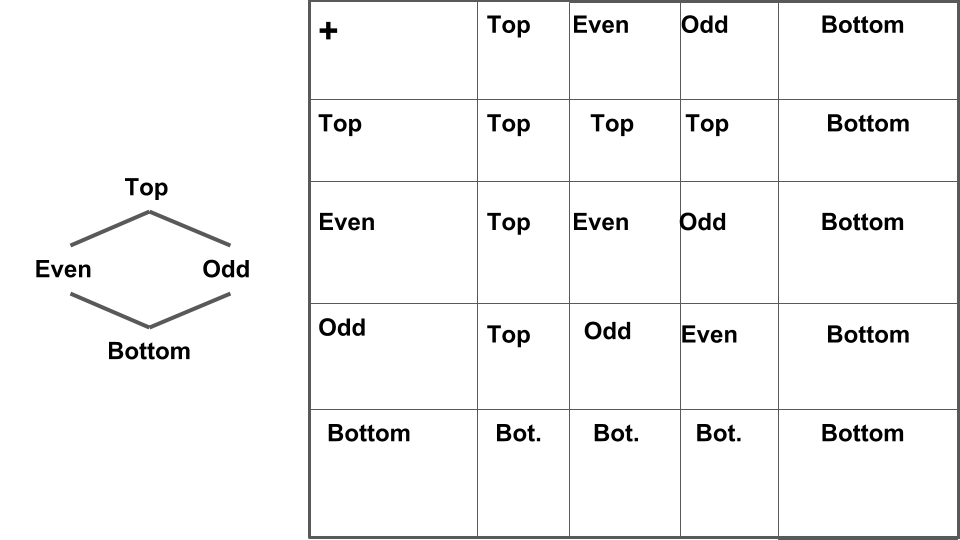
\includegraphics[width=\linewidth]{parity.png}
 \caption{A lattice of abstract domains and a transfer function
   for plus, for an abstract analysis that tracks the parity of
 a value.}
\label{fig-parity}
\end{figure} 

A static analysis can be formally modelled
as a lattice of \textit{abstract domains} and a set of \textit{transfer functions}
that transform abstract domains to other abstract domains when some
program operator is encountered~\cite{cousot77}. The analysis then proceeds by symbolically
interpreting the program being analyzed, replacing each concrete value with
an abstract domain determined by applying the transfer functions. An example
lattice and transfer function for the plus operator are given in Figure~1.
The analysis shown in Figure~1 is a parity analysis---it keeps track of
whether integers are even or odd. There are also two other possiblities:
the integer could be either even or odd (the ``top'' type) or it could
be \textit{both} even and odd---such as in dead code (represented by the
``bottom'' type). The lattice shows how these abstract domains are related,
with a subset relationship represented by the lines---any abstract domain
with a line going to another abstract domain higher in the lattice is a strict
subset of the higher abstract domain (so, for instance, top contains both
all even integers and all odd integers, so both even and odd are below it in the lattice).
The transfer function shows how the result of the plus operation is related
to its operands. We represent this as a matrix, with the top row and leftmost
column representing the abstract domains of the operands, and the interior
parts of the matrix representing the abstract domain of the result. So,
as an example, if $a$ is odd and $b$ is bottom, then $a + b$ is bottom,
because the entry for odd and bottom in the matrix is bottom.

\subsection{Synthesis}

The field of program synthesis uses SMT solvers to
automatically build programs based on a set of constraints provided
by the programmer. Modern SMT solvers, such as z3~\cite{z3}, are able
to solve equations involving millions of variables extremely quickly, despite 
the problem they solve (boolean satisfiabilty) being known to be NP-complete~\cite{cook71complexity}. 
These modern solvers allow the synthesis of, for example, memory models for modern architectures
in a few seconds from the architecture's litmus tests~\cite{bornholt17}.
Synthesis works by reducing the constraints provided by the user
(litmus tests, a formal specification, etc.) to a boolean satisfiability
problem, calling the solver, and then translating the result back into
a program. Because the search space for programs is so large, practical
synthesis techniques use \textit{sketches} of the solution to reduce
the search space. A sketch is an outline of the form of the answer,
such as a program with some expressions missing.

\section{Technical Approach}

\begin{figure}
 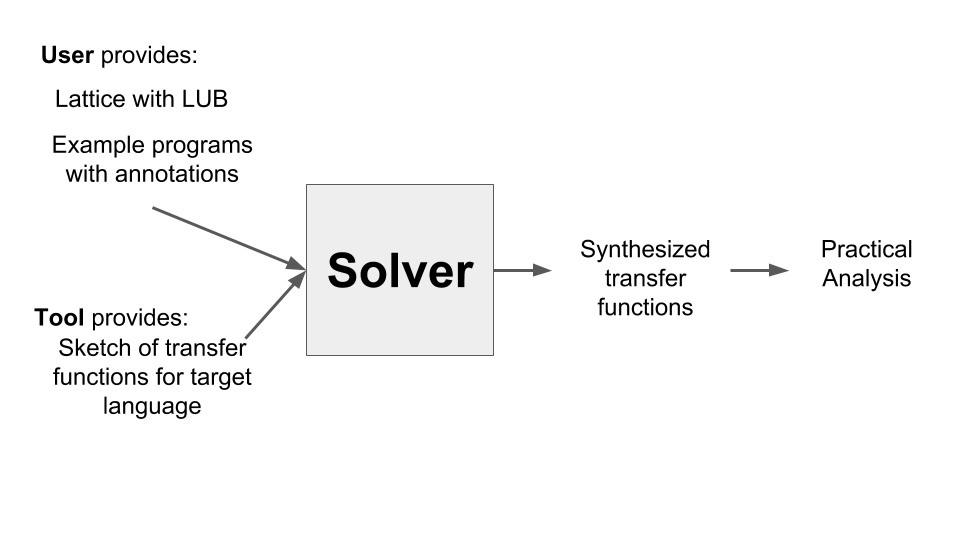
\includegraphics[width=\linewidth]{arch.png}
 \caption{The proposed architecture for the tool.
   Examples are translated to contraints and a sketch of the transfer function is built.
   These are passed to a solver, and then the resulting transfer function is translated into
 a practical analysis.}
\label{fig-arch}
\end{figure} 

Our proposed approach involves three steps.
First, translate examples of the static analysis on sample programs
into constraints on the transfer function and create
a sketch of the transfer functions for the target language.
Constraints are generated by symbolically executing annotated
code examples provided by the programmer in the target language.
Second, pass those constraints and the sketch to the solver;
the result of that solver call is a filled-in transfer
function. Finally, translate the produced transfer function
into an actual analysis that can be run by a programmer.
A diagram of this architecture is shown in \figref{arch}.

The lattice for the abstract analysis is provided by
the programmer, since it must be known to write the examples.
The examples would take the form of code annotated with the
abstract domains (in the same way typed languages have type annotations).
The produced transfer function, along with the known lattice,
contains enough information to mechanically create the practical
analysis on top of a framework like the
Checker Framework~\cite{checker-framework} or LLVM~\cite{lattner04:_llvm}.

The main benefit of our approach is that it relieves the burden of
writing the transfer function from the programmer. The programmer
only needs to write a few slices of annotated code and to provide
the lattice points---even the meaning of the lattice points (i.e. the least
upper bound function) can be inferred from the examples. Instead of
needing to write a lot of code in a possibly unfamiliar framework
(i.e. the backend being used by our tool), the program only needs to
write test cases in the language being analyzed---which is the langauge
they are already working in! Further, actually writing the analysis
would require testing it, and our tool's input is exactly the test
cases a conscientious analysis developer would want to write.

\section{Implementation}

We propose to target the IMP programming language~\footnote{https://www.seas.upenn.edu/~cis500/current/sf/Imp.html}
during this course project, with the idea that we would be able to re-use the internals
(i.e. the code that calls the solver) if the project is successful in
a version of the tool that targetted a more practical language like Java.
We will use z3~\cite{z3} as our solver, and transform the IMP programs directly
into SMT2 constraints using a modified IMP interpreter to symbolically evaluate
the examples. Because of the (time) constraints of a course project, we will not
implement the last stage of our proposed approach, but rather stop with a
synthesized transfer function (there is also little practical value in building
a backend for IMP).

\section{Evaluation}

\begin{table}
\centering
 \begin{tabular}{l c c c c }
  
  Analysis & Test Cases & Precision & Recall & F-measure\\ 
  \midrule
  Parity0 & - & - & - & - \\
  Parity1 & - & - & - & - \\
  ... & - & - & - & - \\
  Sign0 & - & - & - & - \\
  Sign1 & - & - & - & - \\
  ... & - & - & - & - \\
  NPE0 & - & - & - & - \\
  NPE1 & - & - & - & - \\
  ... & - & - & - & - \\
  Range0 & - & - & - & - \\
  Range1 & - & - & - & - \\
  ... & - & - & - & - \\
 \end{tabular}
 \caption{Evaluation of synthesized transfer functions compared
 to ground truth transfer functions. Different analyses with
 the same name but a different number have the same ground truth
 but use a different set of test cases. The analyses are ordered
 by the number of test cases they used. Precision, recall, and
 F-measure are calculated in the standard way against the ground
 truth transfer function.}
 \label{tab-analyses}
\end{table}

We will evaluate our approach by comparing the synthesized transfer
functions for several analyses to the ground truth accepted transfer
functions. The analyses we will consider are: a parity analysis,
a signedness analysis, a null-pointer analysis (using a version of
IMP augmented with a heap), and a range analysis, in that order.

\tabref{analyses} contains a skeleton of our proposed evaluation.
Each row in the table corresponds to a generated set of transfer functions.
For instance,
the row labeled ``Parity0'' states that it is a parity analysis
(from the name), that it was synthesized from $FIXME$ test cases,
and its precision, recall, and F-measure when compared to the ground
truth transfer functions were $FIXME$, $FIXME$, and $FIXME$, respectively.
The ground truth transfer functions were created manually by the authors,
but follow the established standards for their respective analyses.
Precision, recall, and F-measure were calculated following the standard
procedure: precision is the percentage of transfer function entries
in the synthesized transfer function that also appear in the ground truth,
recall is the percentage of transfer function entries in the ground truth
that appear in the synthesized transfer function, and F-measure is the
geometric mean of precision and recall.

Our goal is to achieve a $1.0$ F-measure on at least the parity analysis.
However, it will be interesting to see how many test cases are needed to
reach that goal, which is why we include the weaker analyses we generate
in the table. Since this is exploratory research, our primary goal here
is to just show that this is possible, not to demonstrate that our tool
is superior to the state of the art in any way. That will come later;
see \secref{fw}.

\section{Related Work}

There is a large body of work on abstract interpretation and its relationship
with other, similar static analysis techniques, which is far
too extensive to cover here.
For a sample, see Cousot and Cousot~\cite{cousot14}.
The mathematical framework provided by abstract interpretation is sufficiently
general to express most static analyses, including type systems.
As far as we are aware, this work is the first attempt to automatically
create abstract interpretations from a set of examples, but there is a
large body of prior work that makes building static analysis tools easier.
(whether they are based directly on abstract interpretation or not).
The Checker Framework makes building type systems for Java easier
by providing a framework for type system designers~\cite{checker-framework};
because types are an abstract interpretation, the Checker Framework
is a framework for designing and building abstract interpretations.
IKOS is a framework for developing static analyses directly based on
abstract interpretations, developed by NASA for verifying flight
controllers~\cite{ikos}. Modern compilers use a framework for building
the dataflow analyses they use to perform optimizations and code generation
~\cite{lattner04:_llvm}; these dataflow analyses, too, can be viewed as
abstract interpretations. The current state of the art in industry is to
utilize domain specific query languages to describe static analyses, such as 
Semmle's QL, a datalog variant~\cite{semmle-ql-primer}.
These frameworks and others like them make it easier and faster to develop analyses, but 
building a precise, sound analysis still requires an expert.  Our tool 
aims to remove that requirement by automating the development of analyses; 
we could target our tool to generate code that runs in any of these frameworks.

Previous work on abstract interpretation has considered its relationship
with SAT/SMT solvers, which our approach relies on. Brain et al. characterized
DPLL(T), the main algorithm upon which modern SAT/SMT solvers are built,
as an abstract interpretation~\cite{brain2013abstract}. By calling out to
an SMT solver as part of the transfer function, Jiang et al. are able to
improve the refinements made by their abstract
interpretations~\cite{jiang2017block}. The PAGAI static analyzer uses
an SMT solver to more precisely refine path conditions~\cite{pagai}.
While all of these results combine abstract interpretations with
an SAT or SMT solver in some way, none actually use the solver to
synthesize the abstract interpretation.

A similar domain is inferring invariants. Verifying a program is straightforward
(and can be mechanized~\cite{hoare69}) if inductive invariants are supplied for
each loop or recursive function, and generating these invariants is
known to be a synthesis problem. Recent work has focused on learning
invariants via a counter-example guided approach~\cite{garg2014ice} or
on guessing invariants via an efficient random search algorithm and then
checking whether they are correct~\cite{sharma2016invariant}.
These approaches still require the programmer to specify the correctness
properties of the system formally; our tool allows developers to specify
the analysis they need with examples. In practice, developers write
test cases like the ones our tool requires, but rarely formally specify
the properties of their systems.

Our approach relies on example-driven synthesis, which has been effectively
applied in other domains. Microsoft's Excel spreadsheet tool can automatically
synthesize programs to transform user input based on a few examples
provided by the user using FlashFill~\cite{flashfill}. Bornholt and
Torlak used litmus tests to synthesize memory models for complex architectures
like x86 and PowerPC~\cite{bornholt17}. Perelman et al. developed a general
framework for synthesizing programs from test cases~\cite{perelman2014test}.
These approaches (and ours) share a general framework: the user provides
some examples of what they are trying to accomplish, and a program
(whether it manipulates a spreadsheet, models the memory architecture of
a processor, or implements an abstract interpretation) is produced
automatically by a solver. Our technique extends approaches like these
to a promising new domain: abstract analyses.

\section{Future Work}
\label{sec-fw}

A conference-length paper on this topic would extend the tool to operate
on Java programs, with the final goal being the replication of
existing Checker Framework checkers using only those checkers'
test suites. This would require building signficantly more
complex transfer functions---and probably would require
a meta-sketching approach~\cite{metasketching} which tries several levels of
sketches for the transfer functions (moving from refining only the result of the expression, to
refining multiple variables, to a flow-sensitive refinement, etc.).
This would also require implementing the last stage of the tool, which
translates the synthesized transfer function into a Checker Framework
checker or some other backend.

\section{References}

\begingroup
\renewcommand{\section}[2]{}%

% The following two commands are all you need in the initial runs of
% your .tex file to produce the bibliography for the citations in your
% paper.
\bibliographystyle{plain}
\bibliography{genprog-bib/merged}
% You must have a proper ``.bib'' file
% and remember to run:
% latex bibtex latex latex
% to resolve all references
%
% ACM needs 'a single self-contained file'!
%
\endgroup

\end{document}
This is never printed
